%!TEX root = ../thesis.tex
% ******************************* Thesis Appendix B ********************************

\chapter{Timing Distribution At SBND} 
\label{appendix_timing_dist}
\ifpdf
    \graphicspath{{Appendix3/Figs/Raster/}{Appendix3/Figs/PDF/}{Appendix3/Figs/}}
\else
    \graphicspath{{Appendix3/Figs/Vector/}{Appendix3/Figs/}}
\fi


\begin{figure}[b!] 
\centering    
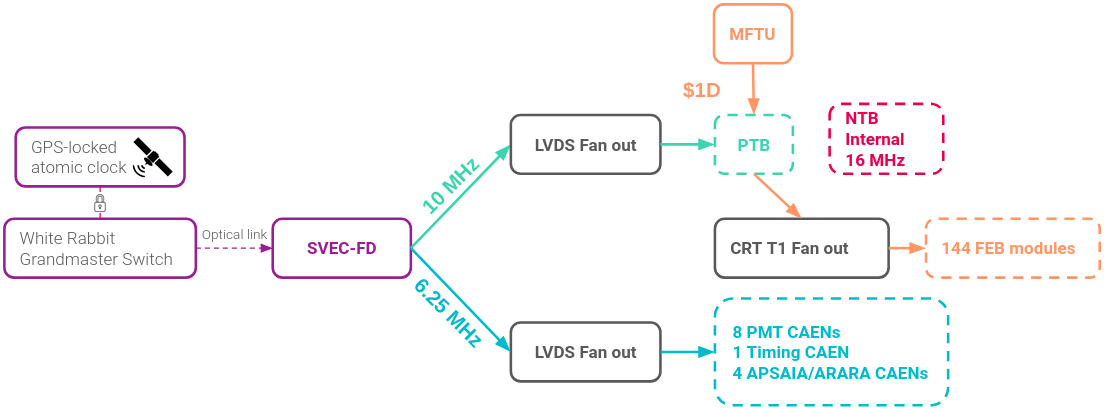
\includegraphics[width=1.0\textwidth]{clock_dist}
\caption[Clock Signal Distribution]{
Clock signal distribution from the White Rabbit timing system to the DAQ subsystems. 
}
\label{fig:clock_dist}
\end{figure}

The White Rabbit (WR) timing system at SBND was previously detailed in Chapter \ref{ChapterDAQ} Sec. \ref{subsec41TimeRef}.                                            
The signal distribution from the WR system is detailed here.                                                                                                           
Fig. \ref{fig:clock_dist} illustrates the clock distribution across the DAQ components.                                                                                
Starting from the SVEC-FD module, two clock frequencies are generated: (1) 10 MHz and (2) 6.25 MHz, shown by the green and blue arrows respectively.
The 10 MHz clock signal is directed through an LVDS fan out, and input to the Penn Trigger Board, as shown by the green box.
The 6.25 MHz clock signal is directed through a LVDS fan out, and distributed in a fan out mode to all CAEN digitisers, as shown by the blue box.                      
Moreover, the PTB also propagates the Beam Early Signal (BES) from the Multi-Function Timing Unit (MFTU), as shown by the solid orange arrow and box.                  
The BES signal is delayed by the PTB, and directed to a CRT T1 fan out module to make multiple copies, which are all input to the FEB modules, as shown by the dashed orange box.                                                                                                                                                             
The Nevis Trigger Board (NTB), as shown by the red box, is the only readout component that does not receive an external clock.                                         
It instead uses an internal clock of 16 MHz.                                                                                                                           

Fig. \ref{fig:pps_dist} shows the distribution of the Pulse Per Second (PPS) signal.
The PPS is first generated by the SVEC-FD and input to fan out modules to make multiple copies.
The copies are distributed to the PTB, CAEN digitisers and FEB modules.
The NTB is a special case, where it receives the PPS from the PTB, where the TTL PPS signal is shifted to a NIM signal.

\begin{figure}[hb!] 
\centering    
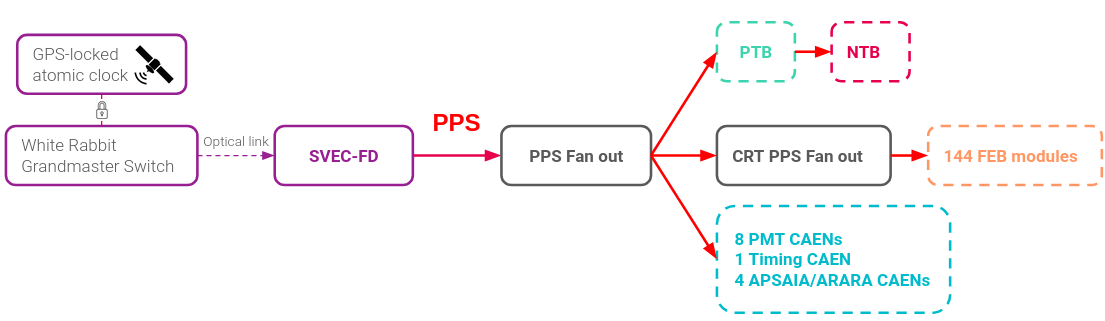
\includegraphics[width=1.0\textwidth]{pps_dist}
\caption[PPS Signal Distribution]{
PPS signal distribution from the White Rabbit timing system to the DAQ subsystems. 
}
\label{fig:pps_dist}
\end{figure}
